\appendix
\section*{Supplementary material}
\renewcommand{\thefigure}{S\arabic{figure}}\setcounter{figure}{0}
\renewcommand{\thetable}{S\arabic{table}}\setcounter{table}{0}

\begin{figure}[h]
\centering
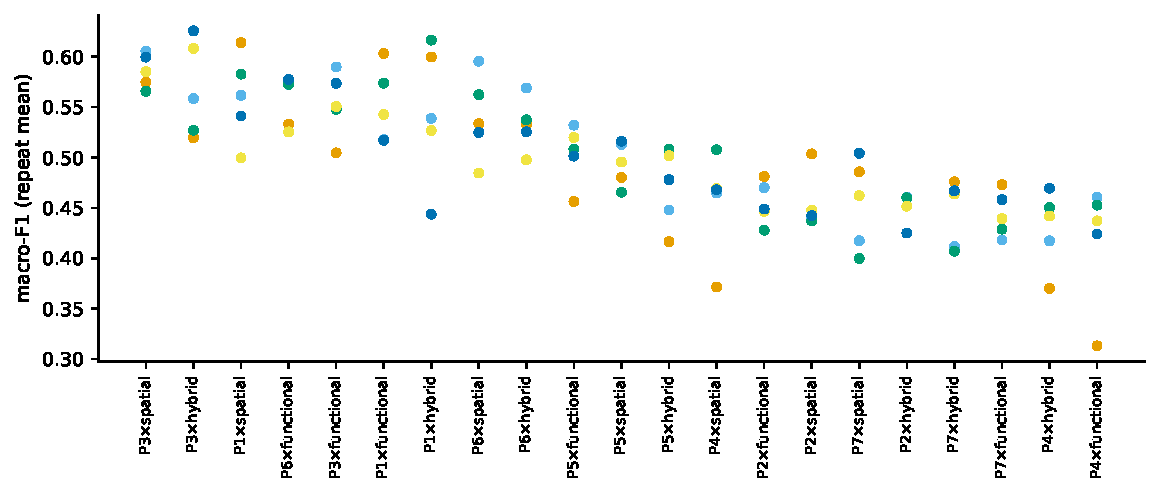
\includegraphics[width=\linewidth]{figS3_seed_variance}
\caption{Mean macro-F1 of each repeat (seed) for every cell on the selection folds: variation due to
the cross-validation partition and initialisation.}
\label{fig:seeds}
\end{figure}

\begin{figure}[h]
\centering
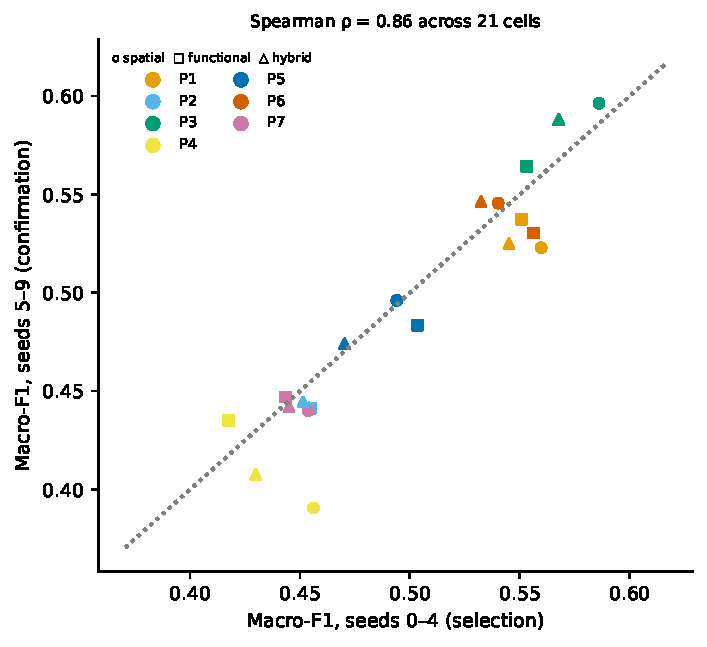
\includegraphics[width=0.75\linewidth]{figS6_confirmation}
\caption{Every cell's mean macro-F1 on the selection folds (seeds 0--4) against the independent
confirmation folds (seeds 5--9); dashed line, identity. Rank correlation: Spearman
$\rho=\confRankRho$.}
\label{fig:confirm}
\end{figure}

\begin{figure}[h]
\centering
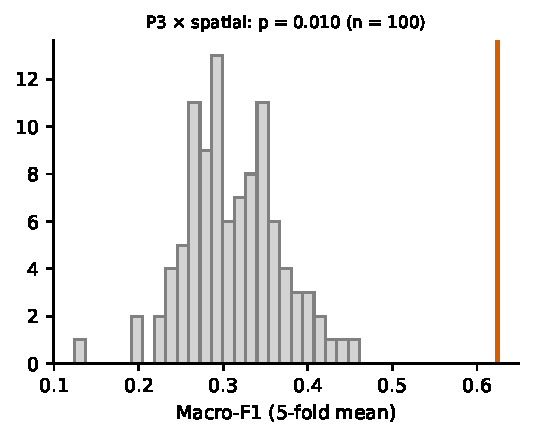
\includegraphics[width=0.5\linewidth]{figS5_permutation_null}
\caption{Label-permutation null distribution (\cpermPThreespatialN{} permutations, first confirmation
repeat's five folds) for the best cell; red line, observed macro-F1 on the same splits.}
\label{fig:perm}
\end{figure}

\begin{table}[h]
\centering\scriptsize
\caption{Paired comparison of each representation's best GCN cell with its best non-graph twin under
both training regimes (25 selection splits). $\Delta$: GCN minus classical; $p$: Holm-corrected
Wilcoxon and Nadeau--Bengio tests within each regime.}
\label{tab:fair}
\setlength{\tabcolsep}{3pt}
\begin{tabular}{lllcccccc}
\toprule
Regime & Representation & GCN & Classical & GCN F1 & Classical F1 & $\Delta$ & $p_\mathrm{W}$ & $p_\mathrm{NB}$ \\
\midrule
\inputtab{generated/tab/fair.tex}
\bottomrule
\end{tabular}
\end{table}

\begin{table}[h]
\centering\scriptsize
\caption{Ablations on the selection folds (seeds 0--4), on which the two reference cells were chosen;
layout as Table~\ref{tab:ablations}. These estimates are subject to selection bias and are given for
comparison only.}
\label{tab:ablations-main}
\begin{tabular}{lcccc}
\toprule
 & \multicolumn{2}{c}{P3 $\times$ spatial} & \multicolumn{2}{c}{P3 $\times$ hybrid} \\
\cmidrule(lr){2-3}\cmidrule(lr){4-5}
Ablation & $\Delta$ [95\% CI] & $p_\mathrm{Holm}$ & $\Delta$ [95\% CI] & $p_\mathrm{Holm}$ \\
\midrule
\inputtab{generated/tab/ablations_main.tex}
\bottomrule
\end{tabular}
\end{table}

\begin{figure}[h]
\centering
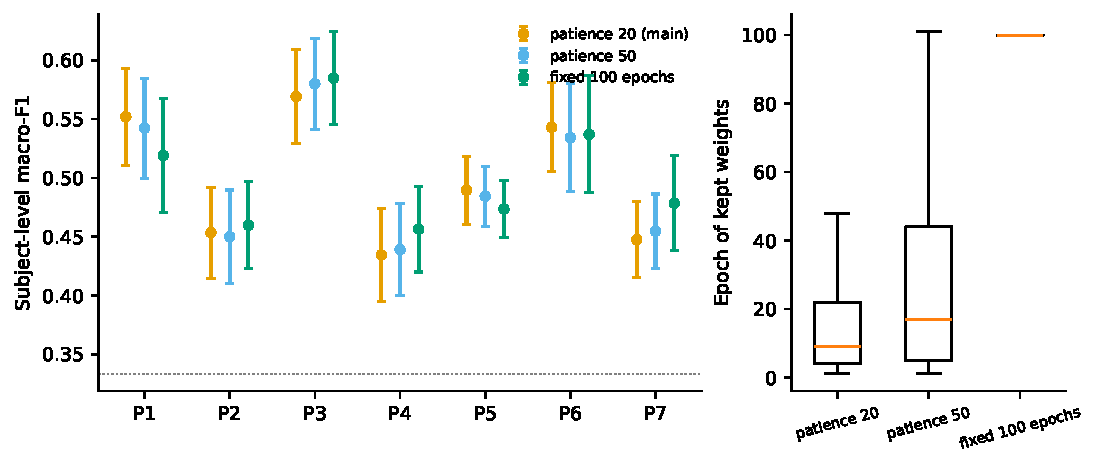
\includegraphics[width=0.9\linewidth]{figS7_early_stopping}
\caption{Stopping-rule sensitivity: macro-F1 per representation (mean and 95\% CI over the 25 selection
splits, averaged over graph types) under each stopping rule (left) and the epoch of the kept weights
(right).}
\label{fig:es}
\end{figure}

\begin{table}[h]
\centering\scriptsize
\caption{Per-representation macro-F1 under each stopping rule (selection splits, averaged over graph
types): change from the main grid and Holm-corrected Wilcoxon $p$ (paired over the 25 splits).}
\label{tab:es-rep}
\begin{tabular}{lccccccc}
\toprule
 & Patience 20 & \multicolumn{3}{c}{Patience 50} & \multicolumn{3}{c}{Fixed 100 epochs} \\
\cmidrule(lr){3-5}\cmidrule(lr){6-8}
Representation & Macro-F1 & Macro-F1 & $\Delta$ & $p_\mathrm{Holm}$ & Macro-F1 & $\Delta$ & $p_\mathrm{Holm}$ \\
\midrule
\inputtab{generated/tab/es_rep.tex}
\bottomrule
\end{tabular}
\end{table}

\begin{figure}[h]
\centering
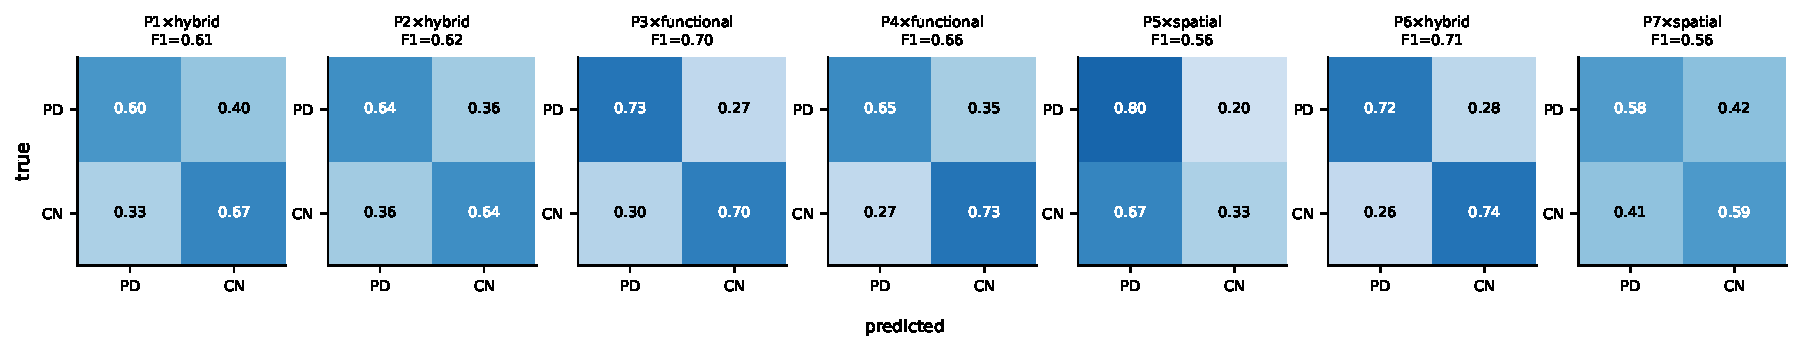
\includegraphics[width=\linewidth]{figS8_external_confusion}
\caption{External cohort ds004584: row-normalised confusion matrices (summed over the 25 test splits)
of the best graph type for each representation.}
\label{fig:ext-confusion}
\end{figure}
